\chapter{Amines et composés azotés}\label{ch:b2:amines}

Le poisson qui n'est plus frais sent la triméthylamine, une petite amine volatile. Un filet de
citron fait disparaître l'odeur~: l'acide protone l'amine, et l'ion ammonium formé, étant un
ion, ne peut pas s'évaporer. Le doublet non liant de l'azote fait des amines des bases et des
nucléophiles~; lié à un carbonyle, il donne les \omterm{def:b2:amines:imine}{imines}, par lesquelles les protéines mènent leur
chimie et les chimistes préparent des amines~; et, sur un cycle \omterm{def:b2:huckel:aromatic}{aromatique}, il ouvre, par les
sels de diazonium, la voie des colorants azoïques qui ont coloré le \textsc{xix}\textsuperscript{e}~siècle.

\begin{recall}
Le volume de première année~: acides et bases de Brønsted, $\mathrm pK_a$ et diagrammes de
prédominance, nucléophiles et substitution bimoléculaire, hémiacétals et acétals, donneurs
d'hydrure, organomagnésiens, classe d'un carbone. \Cref{ch:b2:aromatic-substitution}~:
nitration, réduction des nitroarènes. Le volume scolaire~: amines et amides.
\end{recall}

\begin{omfigure}
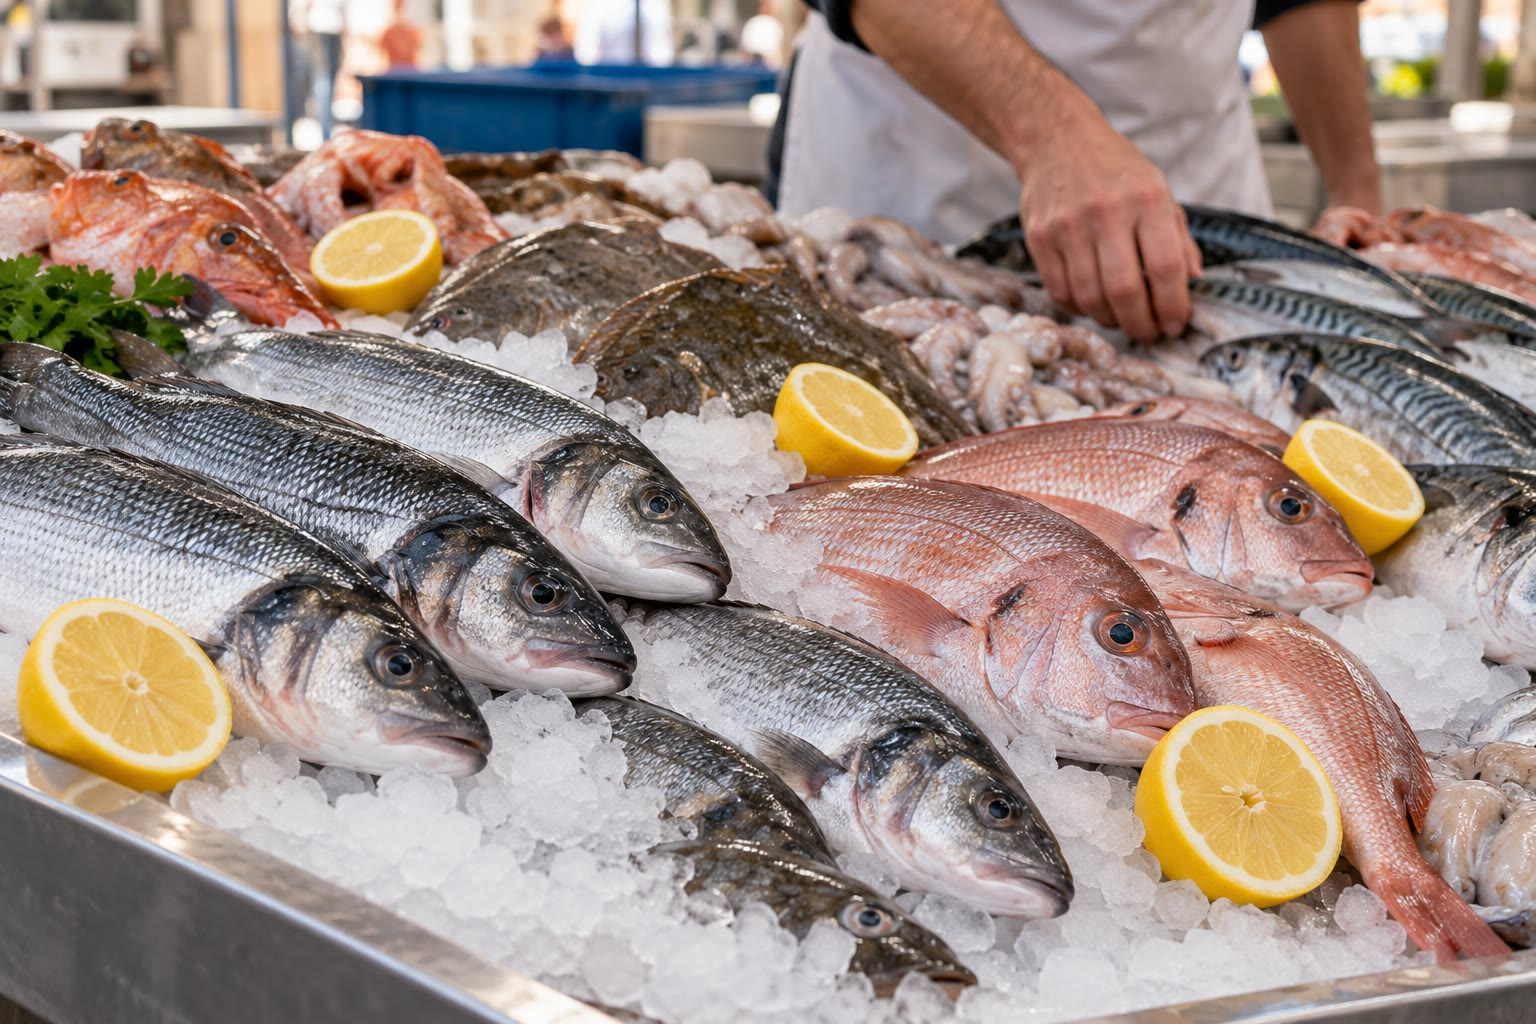
\includegraphics[width=0.6\linewidth]{images/book3/ai/b2-23-fish-stall.jpg}

{\small Un étal de poissonnier~: des moitiés de citron sont disposées parmi les poissons. Leur
acide transforme la triméthylamine du poisson en son ion ammonium, non volatil.}
\end{omfigure}

\section{Structure et basicité}

\begin{definition}[Classes d'amines]\label{def:b2:amines:class}
Une amine est une \emph{amine primaire}\index{amine primaire} \ce{RNH2}, une \emph{amine secondaire}\index{amine secondaire}
\ce{R2NH} ou une \emph{amine tertiaire}\index{amine tertiaire}
\ce{R3N} selon le nombre de groupes carbonés liés à l'azote. Un \emph{ion ammonium
quaternaire}\index{ion ammonium quaternaire} \ce{R4N+} en porte quatre, et aucun doublet non liant.
\end{definition}

L'azote d'une amine est à peu près tétraédrique, le doublet non liant occupant la quatrième
position. Une \omterm{def:b2:amines:class}{amine tertiaire} portant trois groupes différents est chirale en principe mais ne
peut pas être dédoublée~: la molécule s'inverse en passant par une disposition plane, comme un
parapluie retourné par le vent, des milliards de fois par seconde à température ambiante.

\begin{proposition}[Basicité]\label{prop:b2:amines:basicity}
Dans l'eau, les alkylamines sont des bases plus fortes que l'ammoniac ($\mathrm pK_a$ de leurs ions
ammonium vers 10 à 11, contre 9.26), les arylamines des bases bien plus faibles (anilinium 4.60),
et les amides ne sont presque pas basiques (éthanamide protoné vers $-0.6$).
\end{proposition}

\begin{proof}[Argument]
Les groupes alkyle repoussent la densité électronique vers l'azote (effet inductif) et
stabilisent la charge positive de l'ion ammonium. Dans l'eau, la solvatation par liaisons
hydrogène compte aussi~: un ion qui porte plus de liaisons \ce{N-H} est mieux solvaté, ce qui
explique que le triméthylammonium (9.80) soit un acide plus faible que l'ammonium mais plus fort
que le diméthylammonium (10.73). Dans l'aniline, le doublet est délocalisé dans le cycle et se
perd lors de la protonation~; dans un amide, il est délocalisé vers l'oxygène du carbonyle, et la
protonation se fait, faiblement, sur l'oxygène.
% ledger: kb:NH3, pka:methylammonium, pka:dimethylammonium, pka:trimethylammonium, pka:anilinium, pka:ethanamideH
\end{proof}

\begin{omfigure}
\begin{tikzpicture}[font=\small, x=0.85cm]
  \draw[->, thick] (-1.5,0) -- (11.8,0) node[below right] {$\mathrm pK_a$};
  \foreach \x in {0,2,4,6,8,10} \draw (\x,0.1) -- (\x,-0.1) node[below, font=\scriptsize] {\x};
  \foreach \x/\l in {-0.6/{\ce{CH3CONH3+}}, 4.60/{\ce{C6H5NH3+}}} {
    \draw[omDef, thick] (\x,0) -- (\x,0.5);
    \node[font=\scriptsize, anchor=south] at (\x,0.5) {\l};
  }
  \foreach \x/\l/\y/\h in {9.26/{\ce{NH4+} (9.26)}/1.95/1.2, 9.80/{\ce{(CH3)3NH+} (9.80)}/1.45/0.85, 10.66/{\ce{CH3NH3+} (10.66)}/0.95/0.5, 10.73/{\ce{(CH3)2NH2+} (10.73)}/0.45/0.25} {
    \draw[omDef, thick] (\x,0) -- (\x,\h);
    \draw[black!40] (\x,\h) -- (12.2,\y);
    \node[font=\scriptsize, anchor=west] at (12.2,\y) {\l};
  }
  \node[font=\scriptsize, anchor=north west] at (-1.4,-0.5) {bases plus faibles};
  \node[font=\scriptsize, anchor=north east] at (11.7,-0.5) {bases plus fortes};
\end{tikzpicture}

{\small $\mathrm pK_a$ des acides conjugués de quelques bases azotées à
\qty{25}{\degreeCelsius}~: plus il est élevé, plus la base est forte.}
% ledger: kb:NH3, pka:methylammonium, pka:dimethylammonium, pka:trimethylammonium, pka:anilinium, pka:ethanamideH
\end{omfigure}

\section{Les amines, nucléophiles}

Les amines attaquent les halogénoalcanes par substitution bimoléculaire. Le produit, une amine
plus substituée, est au moins aussi nucléophile que l'amine de départ et lui dispute
l'halogénoalcane~: l'alkylation de l'ammoniac donne un mélange d'\omterm{def:b2:amines:class}{amines primaire}, secondaire et
tertiaire et du sel quaternaire.

\begin{proposition}[Polyalkylation]\label{prop:b2:amines:polyalkylation}
L'alkylation directe de l'ammoniac ou d'une \omterm{def:b2:amines:class}{amine primaire} donne des mélanges~; seule
l'alkylation exhaustive jusqu'au sel d'ammonium quaternaire est propre.
\end{proposition}

\begin{proof}[Argument]
Chaque alkylation laisse un doublet non liant sur un azote enrichi en électrons par le nouveau
groupe alkyle~; le produit réagit avec l'halogénoalcane restant à une vitesse comparable. La
séquence ne s'arrête que lorsque l'azote n'a plus de doublet, dans \ce{R4N+}.
\end{proof}

Les \omterm{def:b2:amines:class}{amines primaires} exemptes de leurs homologues suralkylés se préparent indirectement~: par la
voie de Gabriel (alkylation de l'azote du phtalimide, qui porte un seul hydrogène acide, puis
libération de l'amine), par réduction d'un \omterm{def:b2:amines:nitrile}{nitrile}, d'un amide ou d'un dérivé nitré, ou par
\omterm{def:b2:amines:reductive-amination}{amination réductrice} (voir plus loin).

\section{Imines et énamines}

\begin{definition}[Addition nucléophile]\label{def:b2:amines:nucleophilic-addition}
Une \emph{addition nucléophile}\index{addition nucleophile@addition nucléophile} sur un groupe carbonyle est l'attaque
d'un nucléophile sur le carbone du carbonyle, qui devient tétraédrique, la liaison $\pi$ de \ce{C=O}
devenant un doublet non liant de l'oxygène.
\end{definition}

\begin{definition}[Hémiaminals, imines et énamines]\label{def:b2:amines:imine}
Une \omterm{def:b2:amines:class}{amine primaire} s'additionne sur un aldéhyde ou une cétone pour donner un \emph{hémiaminal}\index{hemiaminal@hémiaminal}
(un carbone portant \ce{OH} et \ce{NHR})~; sa déshydratation donne une \emph{imine}\index{imine}
$\mathrm{R_2C{=}NR'}$. Une \omterm{def:b2:amines:class}{amine secondaire}, qui ne peut pas former d'imine neutre, donne après déshydratation une
\emph{énamine}\index{enamine@énamine} $\mathrm{R_2C{=}CR{-}NR'_2}$, la double liaison passant sur le carbone voisin.
\end{definition}

\begin{omfigure}
\setchemfig{atom sep=1.9em}
\schemestart
\chemfig{R_2C=O} \+ \chemfig{H_2N-R'}
\arrow{<=>}
\chemfig{R_2C(-[2]OH)-NH-R'}
\arrow{<=>[\ce{H+}][$-$ \ce{H2O}]}
\chemfig{R_2C=N-R'}
\schemestop
\par\vspace{6pt}

{\small Formation d'une \omterm{def:b2:amines:imine}{imine}~: l'\omterm{def:b2:amines:nucleophilic-addition}{addition nucléophile} de l'amine sur le carbonyle donne
l'\omterm{def:b2:amines:imine}{hémiaminal}~; la catalyse acide transforme son \ce{OH} en groupe partant (\ce{-OH2+}), l'eau part et
le doublet de l'azote forme la double liaison \ce{C=N}. Toutes les étapes sont renversables~: l'eau
en excès hydrolyse l'\omterm{def:b2:amines:imine}{imine} en sens inverse.}
\end{omfigure}

\begin{proposition}[pH optimal]\label{prop:b2:amines:imine-ph}
Les \omterm{def:b2:amines:imine}{imines} se forment le plus vite en solution légèrement acide, vers pH 4 à 5.
\end{proposition}

\begin{proof}[Argument]
La première étape exige l'amine libre (son doublet)~; un milieu trop acide protone l'amine
($\mathrm pK_a$ vers 10) et supprime le nucléophile. La déshydratation exige un acide pour
protoner le groupe hydroxyle~; à pH élevé, elle est lente. La vitesse, qui dépend des deux
exigences à la fois, est maximale entre les deux.
\end{proof}

\begin{definition}[Amination réductrice]\label{def:b2:amines:reductive-amination}
Une \emph{amination réductrice}\index{amination reductrice@amination réductrice} transforme un composé carbonylé et une
amine en une amine plus substituée, en formant l'\omterm{def:b2:amines:imine}{imine} (ou l'ion iminium) et en la réduisant dans
le même récipient, le plus souvent par le cyanoborohydrure de sodium \ce{NaBH3CN}.
\end{definition}

\begin{proposition}[Sélectivité de l'amination réductrice]\label{prop:b2:amines:reductive-amination}
Vers pH 6, \ce{NaBH3CN} réduit l'ion iminium bien plus vite que le composé carbonylé, si bien que
l'amine se forme sans que l'aldéhyde ou la cétone soit réduit en alcool.
\end{proposition}

\begin{proof}[Argument]
Le groupe cyano fait de \ce{BH3CN-} un donneur d'hydrure faible, trop faible pour un carbonyle
neutre mais suffisant pour un ion iminium protoné, chargé positivement, bien meilleur électrophile.
\end{proof}

\section{Sels de diazonium}

\begin{definition}[Chimie des diazoniums]\label{def:b2:amines:diazonium}
Un \emph{ion diazonium}\index{ion diazonium} est un cation \ce{R-N+#N}. La \emph{diazotation}\index{diazotation}
transforme une amine \omterm{def:b2:huckel:aromatic}{aromatique} primaire en sel d'aryldiazonium par le nitrite de sodium et un
acide fort à 0--\qty{5}{\degreeCelsius}. Dans une \emph{réaction de Sandmeyer}\index{reaction de Sandmeyer@réaction de Sandmeyer}, un sel de cuivre(I)
(\ce{CuCl}, \ce{CuBr}, \ce{CuCN}) remplace le groupe diazonium par Cl, Br ou CN avec perte de
diazote. Dans un \emph{couplage azoïque}\index{couplage azoique@couplage azoïque}, l'ion diazonium, électrophile faible,
attaque un cycle \omterm{def:b2:huckel:aromatic}{aromatique} activé pour donner un composé azoïque $\mathrm{Ar{-}N{=}N{-}Ar'}$.
\end{definition}

\begin{proposition}[Stabilité des ions diazonium]\label{prop:b2:amines:diazonium}
Les sels d'aryldiazonium se conservent en solution aqueuse froide et peuvent être utilisés~; les
ions alkyldiazonium perdent aussitôt leur diazote.
\end{proposition}

\begin{proof}[Argument]
Le diazote est un excellent groupe partant (une molécule très stable, un grand gain d'entropie).
Pour un groupe alkyle, la perte de \ce{N2} laisse un carbocation, ou l'eau attaque directement~:
l'ion ne survit pas. Un cation aryle est très instable (une orbitale $\sigma$ vide dans le plan du
cycle, non stabilisée par le système $\pi$), et la liaison \ce{C-N} de l'ion aryldiazonium est
renforcée par conjugaison avec le cycle~: à basse température, il subsiste~; chauffé, il se
décompose, l'eau remplaçant le groupe diazonium par \ce{OH}.
\end{proof}

\begin{omfigure}
\begin{tikzpicture}[font=\small, >={Stealth}]
  \node[cyclenode] (d) at (0,0) {\ce{Ar-N2+}};
  \foreach \a/\t/\c in {90/{\ce{Ar-Cl}}/{\ce{CuCl}}, 150/{\ce{Ar-Br}}/{\ce{CuBr}}, 210/{\ce{Ar-CN}}/{\ce{CuCN}},
                        270/{\ce{Ar-OH}}/{\ce{H2O}, à chaud}, 330/{\ce{Ar-H}}/{\ce{H3PO2}}, 30/{$\mathrm{Ar{-}N{=}N{-}Ar'}$}/{\ce{ArH} activé}} {
    \node[cyclenode] (p\a) at (\a:2.6) {\t};
    \draw[->, thick] (d) -- (p\a) node[midway, font=\scriptsize, fill=white, inner sep=1pt] {\c};
  }
\end{tikzpicture}

{\small Réactions d'un sel d'aryldiazonium. Le groupe \ce{N2+} est remplacé par un halogène ou
un cyanure (Sandmeyer, sels de cuivre(I)), par \ce{OH} (eau chaude) ou par H (acide
hypophosphoreux), ou conservé dans un \omterm{def:b2:amines:diazonium}{couplage azoïque}.}
\end{omfigure}

\begin{method}[Voies passant par un sel de diazonium]\label{met:b2:amines:diazonium-routes}
\begin{enumerate}
  \item Utiliser le groupe amino (\omterm{def:b2:aromatic-substitution:directing}{orienteur ortho/para} fort) pour placer d'autres groupes, puis le
        transformer par l'intermédiaire du sel de diazonium.
  \item Le remplacer par H pour obtenir des motifs que la substitution directe ne peut pas donner
        (le 1,3,5-tribromobenzène à partir de l'aniline).
  \item Le remplacer par CN, puis hydrolyser en acide carboxylique~: une voie vers \ce{-COOH} sur un cycle.
\end{enumerate}
\end{method}

\begin{method}[Préparer une amine]\label{met:b2:amines:make-amine}
\begin{enumerate}
  \item \omterm{def:b2:amines:class}{Amine primaire} sur une chaîne alkyle~: voie de Gabriel, ou réduction d'un \omterm{def:b2:amines:nitrile}{nitrile} (qui
        compte un carbone de plus que l'halogénoalcane dont on le tire) ou d'un amide.
  \item \omterm{def:b2:amines:class}{Amine secondaire} ou tertiaire~: \omterm{def:b2:amines:reductive-amination}{amination réductrice} du composé carbonylé adéquat par
        l'amine adéquate.
  \item Amine \omterm{def:b2:huckel:aromatic}{aromatique}~: nitration, puis réduction (fer ou étain en milieu acide, ou
        \omterm{def:b2:alkene-redox:hydrogenation}{hydrogénation catalytique}).
\end{enumerate}
\end{method}

\section{Nitriles}

\begin{definition}[Nitrile]\label{def:b2:amines:nitrile}
Un \emph{nitrile}\index{nitrile} est un composé \ce{R-C#N}, préparé par substitution d'un
halogénoalcane par l'ion cyanure ou par une \omterm{def:b2:amines:diazonium}{réaction de Sandmeyer}.
\end{definition}

\begin{proposition}[Réactions des nitriles]\label{prop:b2:amines:nitrile}
Un \omterm{def:b2:amines:nitrile}{nitrile} est hydrolysé, en milieu acide ou basique, en amide puis en acide carboxylique~; il est
réduit par l'aluminohydrure de lithium en \omterm{def:b2:amines:class}{amine primaire} \ce{RCH2NH2}~; un organomagnésien s'y
additionne une seule fois, et l'hydrolyse de l'\omterm{def:b2:amines:imine}{imine} formée donne une cétone.
\end{proposition}

\begin{proof}[Argument]
Le carbone du \omterm{def:b2:amines:nitrile}{nitrile} est électrophile, comme un carbone de carbonyle~: l'eau (activée par un
acide, ou sous forme d'hydroxyde) s'y additionne, ce qui donne après tautomérie un amide, dont
l'hydrolyse est traitée au \cref{ch:b2:acyl-substitution}. L'hydrure s'additionne deux fois. Un
organomagnésien s'additionne une fois, en donnant un anion d'\omterm{def:b2:amines:imine}{imine} qui ne réagit pas davantage~;
l'eau hydrolyse ensuite l'\omterm{def:b2:amines:imine}{imine} en cétone.
\end{proof}

\begin{safety}{\ghs[5mm]{GHS03}\,\ghs[5mm]{GHS06}\,\ghs[5mm]{GHS08}\,\ghs[5mm]{GHS09}}
L'aniline et la \textit{N},\textit{N}-diméthylaniline sont toxiques par contact cutané~; le
nitrite de sodium est toxique et oxydant~; le cyanoborohydrure de sodium libère du cyanure
d'hydrogène en milieu acide et s'utilise sous hotte. Les sels de diazonium secs peuvent exploser~:
on les garde toujours au froid, en solution, et on les utilise aussitôt.
% ledger: ghs:aniline, ghs:dimethylaniline, ghs:NaNO2, ghs:NaBH3CN, ghs:sulfanilic-acid
\end{safety}

\section{Exercices}

\begin{exercise}[$\star$]\label{exo:b2:amines:1}
Donner la classe de~: la propan-1-amine, la \textit{N}-méthyléthanamine, la triéthylamine, le
chlorure de tétraméthylammonium, l'aniline.
\end{exercise}

\begin{exercise}[$\star$]\label{exo:b2:amines:2}
Classer par basicité croissante~: l'ammoniac, la méthylamine, l'aniline, l'éthanamide.
\end{exercise}

\begin{exercise}[$\star$]\label{exo:b2:amines:3}
Donner l'\omterm{def:b2:amines:imine}{imine} formée à partir de la cyclohexanone et de la méthylamine, ainsi que les conditions.
\end{exercise}

\begin{exercise}[$\star$]\label{exo:b2:amines:4}
À partir du chlorure de benzènediazonium, donner les produits obtenus avec \ce{CuBr}, \ce{CuCN},
l'eau chaude, et le phénol en milieu basique.
\end{exercise}

\begin{exercise}[$\star\star$]\label{exo:b2:amines:5}
Quelle forme de la triméthylamine prédomine à pH 7, et dans quel rapport~? Expliquer le citron,
et comment une amine peut être extraite d'un solvant organique vers l'eau.
\end{exercise}

\begin{exercise}[$\star\star$]\label{exo:b2:amines:6}
Donner l'\omterm{def:b2:amines:imine}{énamine} formée à partir de la cyclohexanone et de la pyrrolidine, et expliquer pourquoi
une \omterm{def:b2:amines:class}{amine secondaire} ne peut pas donner d'\omterm{def:b2:amines:imine}{imine}.
\end{exercise}

\begin{exercise}[$\star\star$]\label{exo:b2:amines:7}
Préparer la \textit{N}-benzylpropan-2-amine \ce{C6H5CH2NHCH(CH3)2} par \omterm{def:b2:amines:reductive-amination}{amination réductrice}~:
donner deux couples de réactifs possibles.
\end{exercise}

\begin{exercise}[$\star\star$]\label{exo:b2:amines:8}
Le benzonitrile réagit avec le bromure d'éthylmagnésium, puis avec un acide aqueux. Donner le produit.
\end{exercise}

\begin{exercise}[$\star\star$]\label{exo:b2:amines:9}
Écrire la synthèse de Gabriel de l'hexan-1-amine et expliquer pourquoi elle ne donne aucune \omterm{def:b2:amines:class}{amine secondaire}.
\end{exercise}

\begin{exercise}[$\star\star\star$]\label{exo:b2:amines:10}
Préparer le 1,3,5-tribromobenzène à partir de l'aniline.
\end{exercise}

\begin{exercise}[$\star\star\star$]\label{exo:b2:amines:11}
Concevoir un colorant azoïque à partir de la 4-nitroaniline et du phénol~: écrire la \omterm{def:b2:amines:diazonium}{diazotation},
le couplage (position et pH), et le produit.
\end{exercise}

\begin{exercise}[$\star\star\star$]\label{exo:b2:amines:12}
L'hydroxyde d'ammonium quaternaire dérivé de la \textit{N},\textit{N}-diméthylbutan-2-amine,
chauffé, donne surtout du but-1-ène. Expliquer cette orientation de Hofmann, opposée à la règle
de Zaïtsev du volume de première année.
\end{exercise}

\section{Problème~: préparation de l'hélianthine}

\begin{problem}[{Problème du week-end --- l'acide sulfanilique et sa \omterm{def:b2:amines:diazonium}{diazotation}, le \omterm{def:b2:amines:diazonium}{couplage
azoïque} avec la \textit{N},\textit{N}-diméthylaniline, l'hélianthine comme indicateur, et le rendement}]
\label{pb:b2:amines:1}
Données~: acide sulfanilique (acide 4-aminobenzènesulfonique) \ce{C6H7NO3S}~; hélianthine (orangé
de méthyle), sel de sodium \ce{C14H14N3NaO3S}~; $\mathrm pK_a$ de la forme acide de l'hélianthine
3.47. Masses molaires (\unit{g/mol})~: C 12.011, H 1.008, N 14.007, O 15.999, Na 22.990, S 32.06.
Opération (données de l'exercice)~: \qty{5.00}{g} d'acide sulfanilique, rendement 80~\%.
% ledger: pka:methylorange, aw:C, aw:H, aw:N, aw:O, aw:Na, aw:S, ghs:sulfanilic-acid, ghs:NaNO2

\medskip
\noindent\textbf{Partie I --- L'acide sulfanilique et la \omterm{def:b2:amines:diazonium}{diazotation}.}
\begin{enumerate}
  \item L'acide sulfanilique existe sous forme d'amphion (zwitterion). Le représenter.
  \item Pourquoi le dissout-on d'abord dans une solution de carbonate de sodium~?
  \item Écrire la formation de l'acide nitreux à partir du nitrite de sodium et de l'acide chlorhydrique.
  \item Écrire la \omterm{def:b2:amines:diazonium}{diazotation} de l'ion 4-sulfonatoanilinium.
  \item Pourquoi conduit-on la réaction à 0--\qty{5}{\degreeCelsius}~?
  \item Quelle quantité de nitrite de sodium faut-il pour \qty{5.00}{g} d'acide sulfanilique~?
  \item Pourquoi recherche-t-on un léger excès de nitrite, et le détruit-on~?
\end{enumerate}

\medskip
\noindent\textbf{Partie II --- Le couplage.}
\begin{enumerate}[resume]
  \item Pourquoi la \textit{N},\textit{N}-diméthylaniline est-elle un bon partenaire~?
  \item Sur quelle position de son cycle l'\omterm{def:b2:amines:diazonium}{ion diazonium} attaque-t-il, et pourquoi~?
  \item Écrire le produit (sous forme de sulfonate).
  \item Pourquoi conduit-on le couplage en solution faiblement acide, et non fortement acide~?
  \item Pourquoi faut-il ensuite rendre la solution basique pour précipiter le sel de sodium~?
  \item Pourquoi l'\omterm{def:b2:amines:diazonium}{ion diazonium} est-il un électrophile faible, qui ne réagit qu'avec les cycles activés~?
\end{enumerate}

\medskip
\noindent\textbf{Partie III --- Un indicateur.}
\begin{enumerate}[resume]
  \item Quelle est la couleur de l'hélianthine en milieu basique, et en milieu acide~?
  \item Où fixe-t-elle un proton~?
  \item Sur quel domaine de pH sa couleur change-t-elle~?
  \item Pourquoi le système conjugué étendu donne-t-il une couleur visible~?
  \item Pourquoi la protonation déplace-t-elle l'absorption~?
\end{enumerate}

\medskip
\noindent\textbf{Partie IV --- Rendement.}
\begin{enumerate}[resume]
  \item Calculer la masse molaire de l'acide sulfanilique.
  \item Calculer celle de l'hélianthine (sel de sodium).
  \item Calculer la quantité d'acide sulfanilique utilisée.
  \item Calculer la masse théorique d'hélianthine.
  \item Quelles pertes expliquent un rendement inférieur à 100~\%~?
  \item Donner la masse d'hélianthine obtenue à partir de \qty{5.00}{g} d'acide sulfanilique avec
        un rendement de 80~\%.
\end{enumerate}
\end{problem}
